\section{RHP-Zeros Control}
During the development of the project it was apparent that using an integrator was necessary to eliminate steady state-error and reduce the effect of non-linearities thanks to the high-gain linearization effect induced by the integrator. Although, this led to some drawbacks, such as low cut-off frequency. This was induced by the fact that we have 2 complex poles near the imaginary axis, which are the cart natural frequencies. One of the best way to design a controller was to introduce two complex zero in order to cancel the effect of those complex poles. Another way was to use positive zeros in our controller.\\ \\
It is well known from the root locus technique that zeros \emph{attract} poles for increasing gain. Then it was observed, that, if we place positive zeros sufficiently near to the real axis, and not too far from the complex poles  aforementioned, those poles with a sufficient gain would fall in a zone where the output signal response of the system would have low overshoot. \\ \\

\begin{figure}[h]
\centering
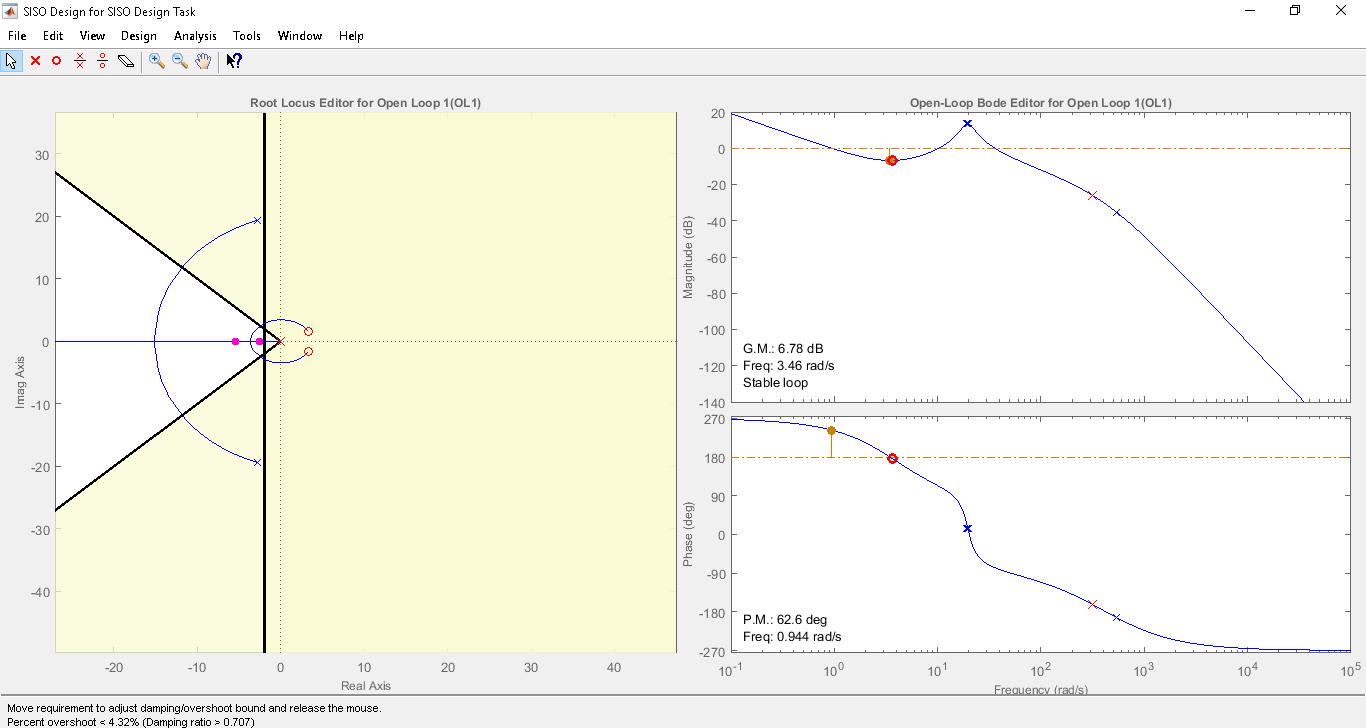
\includegraphics[width=0.5\textwidth]{img/pos_zeros_design.png}
\caption{Root locus and bode plot of the plant with the controller.}
\end{figure}

\begin{figure}[h]
\centering
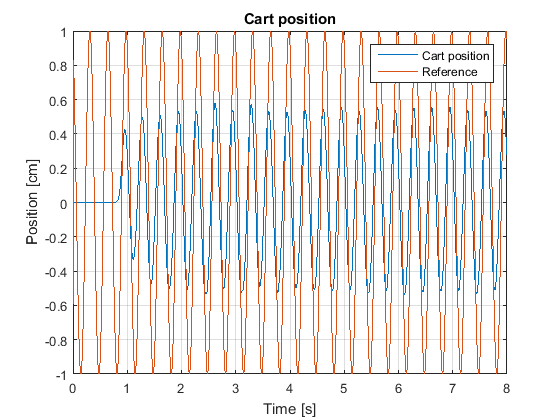
\includegraphics[width=0.5\textwidth]{img/pos_zeros_sin.png}
\caption{Sinusoidal reference tracking. Though the gain is lower that $1$, the phase is almost $0$.}
\end{figure}


  \begin{figure}[!tbh]
  \centering
  \subfloat[ $K_l$]{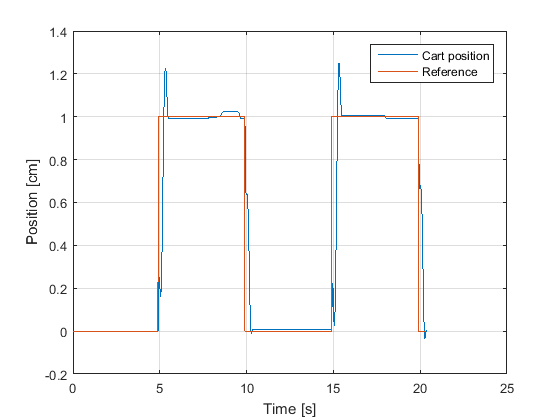
\includegraphics[width=0.5\textwidth]{img/pos_zeros_kh_1.png}}
  \hfill
  \subfloat[ $K_h$]{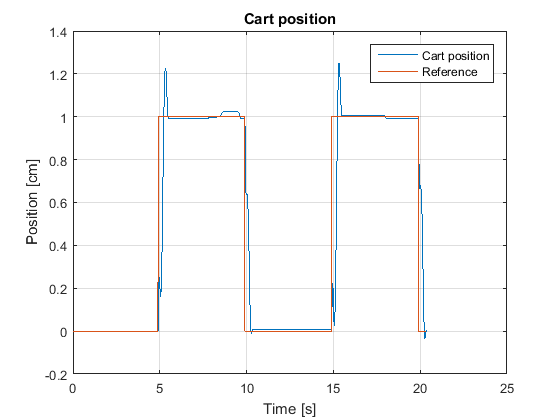
\includegraphics[width=0.5\textwidth]{img/pos_zeros_kh_2.png}}
  \caption{On the left: plot of the cart position with  $K_l$. On the right plot of the cart position with $K_h$.}
    \label{fig:poss}
\end{figure}